\documentclass{article}
\usepackage[utf8]{inputenc}
\usepackage[spanish]{babel}
\usepackage{graphicx}
\usepackage{geometry}
\usepackage{enumerate}
\usepackage{titlesec}
\usepackage{float}
\usepackage{listings}
\usepackage{xcolor}
\usepackage{amsmath}
\usepackage{matlab-prettifier}
\usepackage{amssymb}
\usepackage{tabularx}

\geometry{letterpaper, margin = 1.5cm}

\newcommand{\codefontsize}{\fontsize{10}{11}}
\lstset{
	style = Matlab-editor,
	basicstyle = \codefontsize\ttfamily,
	mlshowsectionrules = true,
	upquote = true,
	tabsize = 4,
	captionpos = b,
	breaklines = true,
	breakatwhitespace = true,
	frame = single,
}

%Datos de la Portada
\title{Introducción a la Programación \ Practica 7}
\author{Medina Martinez Jonathan Jason \ 2023640061}
\date{15 de mayo del 2023}

\begin{document}
	
	\fontsize{12}{16}\selectfont
	
	\begin{figure}[t]
		
		
\includegraphics[width=2.5 cm]{Logo1.jpeg}
		\hfill
		
\includegraphics[width=3 cm]{Logo2.png}
		
	\end{figure}
	
	\maketitle
	\newpage
	
	\tableofcontents
	\newpage
	
	\section{Objetivo}
	
	Conocer los diferentes tipos de controles en las interfaces graficas.
	
	\section{Introducción}
	
	La práctica 7 de Herramientas Computacionales tiene como objetivo brindar una introducción a las interfaces gráficas y explorar los diferentes tipos de controles que se utilizan en ellas. En esta práctica, utilizaremos MATLAB App Designer para crear una aplicación con una interfaz gráfica de usuario que nos permitirá realizar diversas operaciones matemáticas. A través de esta experiencia, podremos comprender cómo diseñar y desarrollar interfaces interactivas que faciliten la interacción del usuario con un programa.
	
	\newpage
	\section{Desarrollo}
	
	Con MATLAB App Designer cree una aplicación con interfaz grafica de usuario que permita realizar las siguientes operaciones:
	
	\begin{itemize}
		\item Suma
		\item Resta
		\item Multiplicación
		\item División
		\item Raíz enésima
		\item Potenciación
		\item Logaritmo base n
	\end{itemize}
	
	\subsection{Calculadora.mlapp}
	
	\subsubsection{Interfaz}
	
	\begin{figure*}[h]
		\centering
		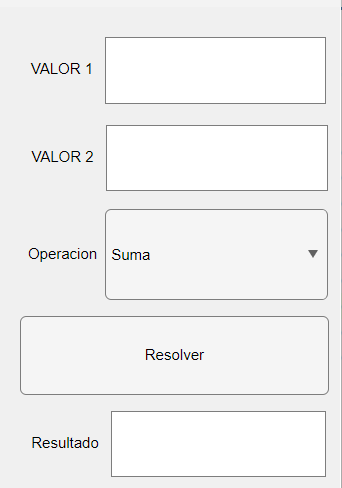
\includegraphics[height = 14cm]{img1.png}
	\end{figure*}
	
	\newpage
	
	\subsubsection{Código}
	
	\begin{lstlisting}
	classdef Calculadora < matlab.apps.AppBase
	
		% Properties that correspond to app components
		properties (Access = public)
			UIFigure                matlab.ui.Figure
			Resolver                matlab.ui.control.Button
			VALOR2EditFieldLabel_2  matlab.ui.control.Label
			Valor2                  matlab.ui.control.EditField
			Operacion               matlab.ui.control.DropDown
			OperacionDropDownLabel  matlab.ui.control.Label
			ResultadoLabel          matlab.ui.control.Label
			Resultado               matlab.ui.control.EditField
			Valor1                  matlab.ui.control.EditField
			VALOR1EditFieldLabel    matlab.ui.control.Label
		end
		
		% Callbacks that handle component events
		methods (Access = private)
		
			% Button pushed function: Resolver
			function ResolverButtonPushed(app, event)
				valor1 = str2double(app.Valor1.Value);
				valor2 = str2double(app.Valor2.Value);
				op = app.Operacion.Value;
				
				switch op
					case 'Suma'
						res = valor1 + valor2;
					case 'Resta'
						res = valor1 - valor2;
					case 'Multiplicacion'
						res = valor1 * valor2;
					case 'Division'
						res = valor1 / valor2;
					case 'Raiz enesima'
						res = nthroot(valor1, valor2);
					case 'Potenciacion'
						res = valor1^valor2;
					case 'Logaritmo base n'
						res = log(valor2) / log(valor1);
				end
	
				app.Resultado.Value = num2str(res);
			end
		end
	
		% Component initialization
		methods (Access = private)
	
		% Create UIFigure and components
		function createComponents(app)
	
		% Create UIFigure and hide until all components are created
		app.UIFigure = uifigure('Visible', 'off');
		app.UIFigure.Position = [100 100 273 394];
		app.UIFigure.Name = 'MATLAB App';
	
		% Create VALOR1EditFieldLabel
		app.VALOR1EditFieldLabel = uilabel(app.UIFigure);
		app.VALOR1EditFieldLabel.HorizontalAlignment = 'center';
		app.VALOR1EditFieldLabel.Position = [15 319 71 55];
		app.VALOR1EditFieldLabel.Text = 'VALOR 1';
	
		% Create Valor1
		app.Valor1 = uieditfield(app.UIFigure, 'text');
		app.Valor1.Position = [85 319 177 53];
	
		% Create Resultado
		app.Resultado = uieditfield(app.UIFigure, 'text');
		app.Resultado.HorizontalAlignment = 'center';
		app.Resultado.Position = [90 20 172 53];
	
		% Create ResultadoLabel
		app.ResultadoLabel = uilabel(app.UIFigure);
		app.ResultadoLabel.HorizontalAlignment = 'center';
		app.ResultadoLabel.Position = [16 20 74 55];
		app.ResultadoLabel.Text = 'Resultado';
	
		% Create OperacionDropDownLabel
		app.OperacionDropDownLabel = uilabel(app.UIFigure);
		app.OperacionDropDownLabel.HorizontalAlignment = 'center';
		app.OperacionDropDownLabel.Position = [16 162 70 73];
		app.OperacionDropDownLabel.Text = 'Operacion';
		
		% Create Operacion
		app.Operacion = uidropdown(app.UIFigure);
		app.Operacion.Items = {'Suma', 'Resta', 'Multiplicacion', 	'Division', 'Raiz enecima', 'Potenciacion', 'Logaritmo base n'};
		app.Operacion.Position = [85 162 178 73];
		app.Operacion.Value = 'Suma';
	
		% Create Valor2
		app.Valor2 = uieditfield(app.UIFigure, 'text');
		app.Valor2.Position = [86 249 177 53];
		
		% Create VALOR2EditFieldLabel_2
		app.VALOR2EditFieldLabel_2 = uilabel(app.UIFigure);
		app.VALOR2EditFieldLabel_2.HorizontalAlignment = 'center';
		app.VALOR2EditFieldLabel_2.Position = [16 249 70 55];
		app.VALOR2EditFieldLabel_2.Text = 'VALOR 2';
		
		% Create Resolver
		app.Resolver = uibutton(app.UIFigure, 'push');
		app.Resolver.ButtonPushedFcn = createCallbackFcn(app, @ResolverButtonPushed, true);
		app.Resolver.Position = [17 86 247 63];
		app.Resolver.Text = 'Resolver';
		
		% Show the figure after all components are created
			app.UIFigure.Visible = 'on';
			end
		end
		
		% App creation and deletion
		methods (Access = public)
		
		% Construct app
		function app = Calculadora
		
		% Create UIFigure and components
		createComponents(app)
		
		% Register the app with App Designer
		registerApp(app, app.UIFigure)
		
			if nargout == 0
				clear app
			end
		end
		
		% Code that executes before app deletion
		function delete(app)
		
		% Delete UIFigure when app is deleted
			delete(app.UIFigure)
			end
		end
	end
	\end{lstlisting}
	
	\subsubsection{Ejemplo 1}
	
	\begin{figure*}[h]
		\centering
		
\includegraphics[height = 8cm]{img2.png}
	\end{figure*}
	
	\subsubsection{Ejemplo 2}
	
	\begin{figure*}[h]
		\centering
		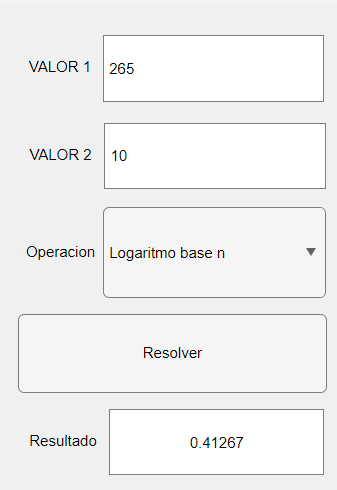
\includegraphics[height = 8cm]{img3.png}
	\end{figure*}
	
	\newpage
	\section{Conclusión}
	
	En conclusión, la práctica 7 de Herramientas Computacionales nos ha brindado una valiosa introducción al mundo de las interfaces gráficas de usuario. Hemos aprendido cómo utilizar MATLAB App Designer para crear una aplicación con una interfaz gráfica intuitiva y amigable, lo que nos ha permitido realizar diversas operaciones matemáticas de manera sencilla y eficiente.
	
	A lo largo de la práctica, se exploran los diferentes tipos de controles disponibles en App Designer, como botones, cajas de texto y menús desplegables, y hemos comprendido cómo utilizarlos para interactuar con el usuario de manera efectiva.
	
\end{document}